\subsection{Player interfaces}
\noindent Field responders are equipped with a `mobile responder tool' providing sensing and awareness capabilities in three tabs (geiger counter, map, messaging and tasks; see figure \ref{fig:ui}). The first tab shows a reading of radioactivity, player health level (based on exposure), and a GPS-enabled map of the game area to locate fellow responders, the targets to be rescued and the drop off zones for the targets. The second tab provides a broadcast messaging interface to communicate with fellow field responders and HQ. The third tab shows the team and task allocation dynamically provided by the agent that can be accepted or rejected. Notifications are used to alert both to new messages and task allocations.

\begin{figure}[htbp]
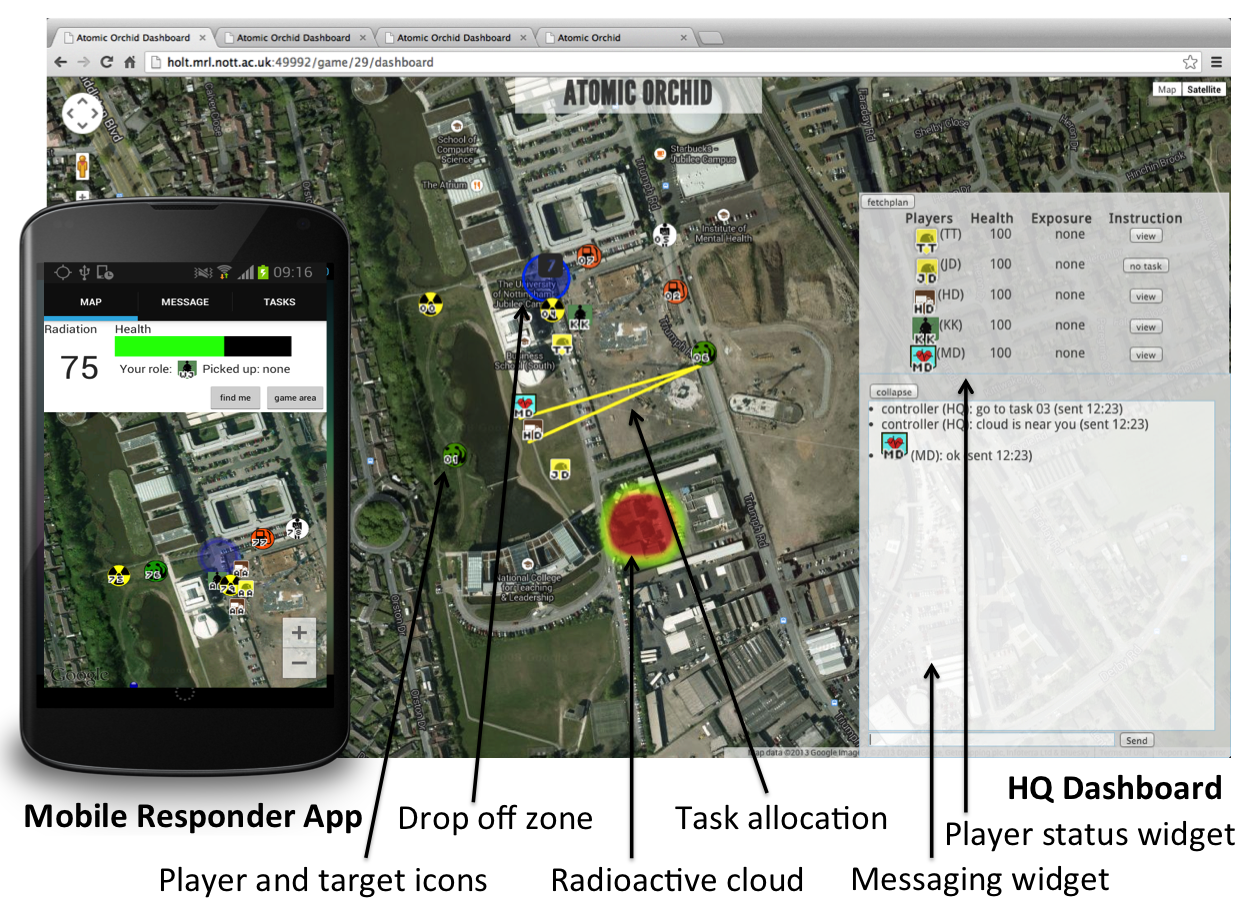
\includegraphics[width=\columnwidth]{UI.png}
\label{fig:ui}
\caption{Mobile field responder and HQ interfaces.\vspace{-3mm}
}\end{figure}

The HQ is manned by at least one player (the HQ commander) who has at her disposal an `HQ dashboard' that provides an overview of the game area, including real-time information of the players' locations (see figure \ref{fig:ui}). The dashboard provides a broadcast messaging widget, and a player status widget so that the responders' exposure and health levels can be monitored. The HQ commander can further monitor the  current team and task allocations by the agent. Crucially, only the HQ has a view of the radioactive cloud, depicted as a heatmap where `Hotter'  (red) zones correspond to higher levels of radioactivity.

\subsection{System architecture}
\noindent AtomicOrchid is based on the open-sourced geo-fencing game MapAttack\footnote{http://mapattack.org} that has been iteratively developed for a responsive, (relatively) scalable experience.  The location-based game is underpinned by client-server architecture, that relies on real-time data streaming between client and server. Client-side requests for less dynamic content use HTTP. Frequent events, such as location updates and radiation exposure, are streamed to clients to avoid the overhead of HTTP. In this way, field responders are kept informed in near real-time. Finally,  to build the mobile app, we adapted an existing MapAttack Android app.

%The platform is built using the geoloqi platform, Sinatra for Ruby, and state-of-the-art web technologies such as socket.io, node.js and the Google Maps API. 

\subsection{Integrating the Planning agent}
\noindent The planning agent as described in Section \ref{sec:algo} takes the game status (i.e., positions of players, known status of the cloud, and messages received from players - see below) as input and produces a plan of optimal coalition to task allocation for the current state. The agent is deployed on a separate server. The AtomicOrchid server requests a plan from the agent via a stateless HTTP interface by transmitting the game status in JSON format. Polling (and thus re-planning) is triggered by two kinds of game events:
\begin{itemize}
\item \textit{Completion of task}. On successful rescue of a target, a new plan (i.e., allocation of tasks to each responder) is requested from the agent.
\item \textit{Explicit reject}. On rejection of a task allocation by field responders, a new plan is requested. More importantly, the rejected allocation is, in turn, used as a constraint within the optimisation run by the planner agent (as described in Section \ref{sec:adaptive}).
\end{itemize} 

%\subsection{Interacting with planning agent}
%There can interact directly with field players through a task tab (Figure xx) and agent plans are also visible to HQ's dashboard interface.
Once a plan is pulled from the planning agent, the AtomicOrchid game engine splits the plan for a given coalition into individual task allocations for each player and send them to their mobile responder app. The app presents the task allocation in the task tab, detailing: 1) the responder to team up with, 2) the allocated target (using target id), and 3) approximate direction of the target (e.g., north, east). 

Once a player accepts a task, an acknowledgement is sent to their teammates, while rejecting a task triggers a task assignment from the agent. Furthermore, the HQ commander is provided with a visualisation of task allocations for each player on demand (by button press), to help monitor the task allocation computed by the agent.

